\documentclass[11pt]{article}
\usepackage{amsmath}
\usepackage{graphicx}
\pagestyle{empty}
\textwidth 6.5in
\textheight 9.0in
\hoffset -1.0in
\voffset -0.75in
\parindent 0pt
\newcommand\eqnumber{\addtocounter{equation}{1}\tag{\theequation}}
\begin{document}
\centerline{\large\bf  N-BODY DECAY CODE}

The code generates $N$ momenta such that
\begin{align*}\eqnumber
dN_p&\sim \frac{d^3p_1}{\epsilon_1}\cdots\frac{d^3p_N}{\epsilon_N}\delta^4(\sum_np_n-P).
\end{align*}
where $P=(M,0,0,0)$ is the momenta of the decaying particle of mass $M$ and the $N$ daughters have masses $m_1\cdots m_N$. The number of configurations within the differential phase space is $dN_p$.

We begin by seeing that 
\begin{align*}\eqnumber
\frac{d^3p_1}{\epsilon_1}\frac{d^3p_2}{\epsilon_2}&=
\frac{d^3\tilde{p}_1}{\tilde{\epsilon}_1}\frac{d^3\tilde{p}_2}{\tilde{\epsilon}_2},
\end{align*}
where the quantities with the tilde are in frame where $\vec{p}_1+\vec{p}_2=\vec{P}_{12}\approx 0$. Defining the relative momenta in that frame as $\tilde{q}_{1;2}=|\vec{p}_1-\vec{p}_2|/2$, one can see that
\begin{align*}\eqnumber
\frac{d^3p_1}{\epsilon_1}\frac{d^3p_2}{\epsilon_2}&=
4\pi \tilde{q}_{1;2}^2d\tilde{q}_{1;2}d^3P_{12}\frac{1}{\tilde{\epsilon}_1\tilde{\epsilon}_2}.
\end{align*}
Next, we define the kinetic energy of the system in this frame, then differentiate it w.r.t. $\tilde{q}_{1;2}$,
\begin{align*}\eqnumber
K_{1;2}&=\tilde{\epsilon}_1+\tilde{\epsilon}_2-m_1-m_2,\\
dK_{1;2}&=\tilde{q}_{1;2}d\tilde{q}_{1;2}\left(\frac{1}{\tilde{\epsilon}_1}+\frac{1}{\tilde{\epsilon}_1}\right)\\
&=\tilde{q}_{1;2}d\tilde{q}_{1;2}\frac{\tilde{\epsilon}_1+\tilde{\epsilon}_2}{\tilde{\epsilon}_1\tilde{\epsilon}_2}.
\end{align*}
This gives
\begin{align*}\eqnumber
\frac{d^3p_1}{\epsilon_1}\frac{d^3p_2}{\epsilon_2}&=
4\pi\tilde{q}_{1;2}dK_{1;2}\frac{d^3\tilde{P}_{12}}{M_{12}},
\end{align*}
where $M_{12}=\tilde{\epsilon}_{12}$ is the invariant mass of the two-particle cluster and 
\begin{eqnarray}
K_{1;2}&=M_{12}-m_1-m_2.
\end{eqnarray}
One can iterate the expression by replacing $2$ with $3$ and $1$ with $12$, thus having the cluster of the first two particles playing the role of the first particle.
\begin{align*}\eqnumber
\frac{d^3p_{12}}{\epsilon_{12}}\frac{d^3p_3}{\epsilon_3}&=
4\pi\tilde{q}_{12;3}dK_{12;3}\frac{d^3\tilde{P}_{123}}{M_{123}},\\
K_{12;3}&=M_{123}-M_{12}-m_3,\\
K_{1;2}+K_{12;3}=M_{123}-m_1-m_2-m_3;
\end{align*}
The expression then becomes
\begin{align*}\eqnumber
dN&=(4\pi)^{N-1}\tilde{q}_{1;2}\tilde{q}_{12;3}\cdots \tilde{q}_{1\cdots n-1;n}\cdots \tilde{q}_{1\cdots N-1;N}\\
&dK_{1;2}dK_{12;3}\cdots dK_{1\cdots N-1;N}\\
&\frac{d^3P_{1\cdots N}}{M_{1\cdots N}}\delta^3(\vec{P}_{1\cdots N})\delta(M-\sum_n\epsilon_n).
\end{align*}
The sum of the kinetic energies are
\begin{align*}\eqnumber
K_{\rm tot}=K_{1;2}+K_{12;3}+K_{123;4}+\cdots K_{1\cdots N-1;N}&=M_{1\cdots N}-\sum_n\epsilon_n.
\end{align*}
Thus, 
\begin{align*}\eqnumber
dN&=\frac{1}{M}(4\pi)^{N-1}\tilde{q}_{1;2}\tilde{q}_{12;3}\cdots \tilde{q}_{1\cdots n-1;n}\cdots \tilde{q}_{1\cdots N-1;N}\\
&dK_{1;2}dK_{12;3}\cdots dK_{1\cdots N-1;N}\\
&\delta(K_{1;2}+K_{12;3}+\cdots K_{12\cdots N-1;N}-(M-\sum_im_i)).
\end{align*}
where each of the momenta are given by the expression
\begin{align*}\eqnumber
\tilde{q}_{I;j}&=\left\{\frac{m_{Ij}^4+M_I^4+m_j^4-2M_{Ij}^2M_I^2-2M_{Ij}^2m_j^2-2M_I^2m_j^2}{4M_{Ij}^2}\right\}^{1/2}.
\end{align*}

{\bf Sampling the Kinetic Energies}\\
An efficient method for sampling the kinetic energies is to
\begin{enumerate}
\item[a)]Choose $N-2$ random numbers uniformly between zero and $K_{\rm tot}=M-\sum_im_i$, plus two values set to zero and $K_{\rm tot}$.
\item[b)] Sort the $N$ values.
\item[c)] Use each of the $N-1$ differences between successive value for $K_{1;2}, K_{12;3}, K_{123;4}\cdots$. The differences sum to $K_{\rm tot}$.
\end{enumerate}
To prove that this sampling represents the integral over $K$ above, one can compare how each approach would give $P(n,x)$, the probability density that the first $n$ values (Not ordered by size) of $K_i$ would sum to $x$, where each value has a uniform probability between $0$ and $K_{\rm tot}$. The target probability distribution is
\begin{align*}\eqnumber
dN&=\left(\frac{1}{K_{\rm tot}}\right)^{N-1}dK_{1;2}dK_{12;3}dK_{123;4}\cdots dK_{1\cdots N-1;N}\delta(K_{\rm tot}-K_{1;2}-K_{12;3}-\cdots K_{N-1;N}).
\end{align*}
If one were to integrate the $n$ values, one can write a recursive relation
\begin{align*}\eqnumber
P(n,x)&=\frac{1}{K_{\rm tot}}\int_0^xdy~P(n-1,y). 
\end{align*}
Given that $P(1,x)=1/K_{\rm tot}$, one can integrate
\begin{align*}\eqnumber
P(2,x)&=\frac{1}{K_{\rm tot}}\int_0^xdy \frac{1}{K_{\rm tot}}\\
&=\frac{1}{K_{\rm tot}}\frac{x}{K_{\rm tot}}.
\end{align*}
Continuing,
\begin{align*}\eqnumber
P(3,x)&=\frac{1}{2}\frac{1}{K_{\rm tot}}\left(\frac{x}{K_{\rm tot}}\right)^2,\\
P(n,x)&=\frac{1}{(n-1)!}\frac{1}{K_{\rm tot}}\left(\frac{x}{K_{\rm tot}}\right)^{n-1}.
\end{align*}
If one applies the algorithm described above, one can see that in order to sum the first $n$ particles to $x$, one must have one of the particles equal $x$, then have the other $n-1$ values less that $x$. This probability is
\begin{align*}\eqnumber
P(n,x)&=\frac{n}{K_{\rm tot}}\left(\frac{x}{K_{\rm tot}}\right)^{n-1}.
\end{align*}
Aside from an overall constant factor, the scaling with $x$ are identical. Thus, the algorithm above faithfully reproduces the distribution. 

{\bf Monte Carlo Weights}\\
However, the desired weight also has the factors
\begin{align*}\eqnumber
w=\tilde{q}_{1;2}\tilde{q}_{12;3}\cdots \tilde{q}_{1\cdots n-1;n}\cdots \tilde{q}_{1\cdots N-1;N}.
\end{align*}
After choosing the $N-1$ $K$ values, one must calculate the product of the  $N-1$ values of $q$. One must then use the $w$ as a weight. For a given set of masses, one can use a keep or reject method to choose the values of $K$ with the complete weights. Unfortunately, this requires knowing the maximum weight so that the keep or reject probability for a given configuration of kinetic energies is $w/w_{\rm max}$. Here, $w_{\rm max}$ is the value of highest value of $w$ one can have for any values of $K_{1;2},K_{12:3}cdots$. If one chooses a value of $w_{\rm max}$ that is higher than the true maximum, the Monte Carlo procedure will still work with perfect accuracy, but the efficiency will suffer. Empirically, it was found that to estimate $w_{\rm max}$ one can first calculate $w$ with each kinetic energy value set to $K_{\rm tot}/(N-1)$. We then multiplied this value by a factor
\begin{align*}
F&=y=1.0+\alpha(n-2)+\beta*\tanh((n-2)/x_0),
\alpha&=0.17, ~\beta=0.415, ~x_0=2.8.
\end{align*}
This is shown as a function of $n$ below.
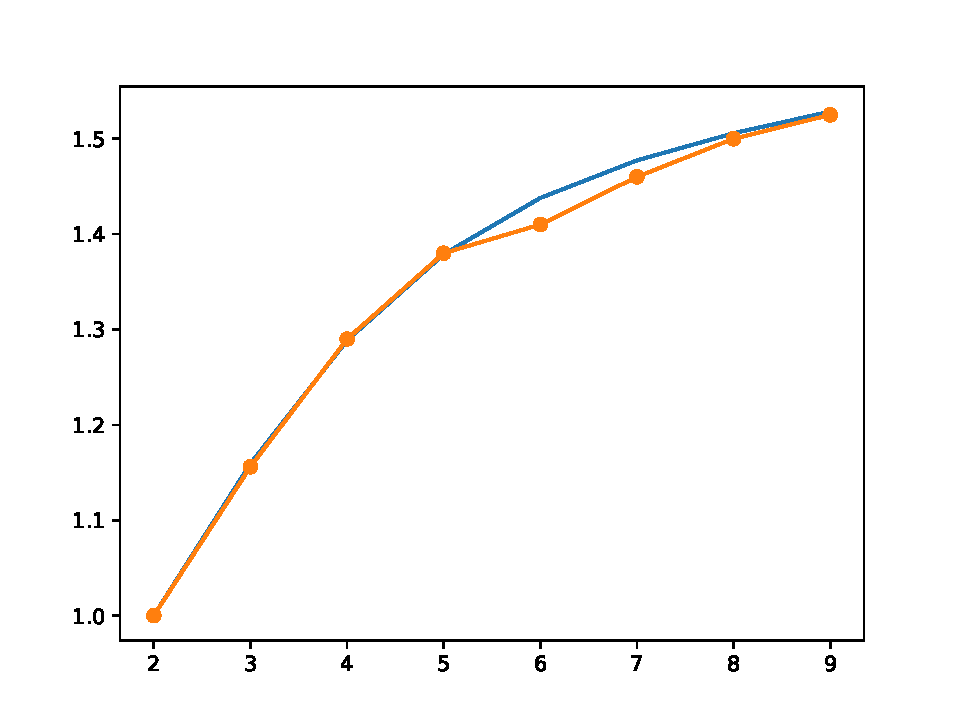
\includegraphics[width=0.5\textwidth]{maxfactor}
The points are the maximum values found by randomly trying billions of masses and billions of values of $K$. For some configuration of masses, the true value of $F$ should be somewhere between unity and the values graphed. It would seem that knowing the true value could only improve the efficiency by a few tens of percent.

One the configuration of $K$ values is accepted, one then generates the $q$ values for each $K$. Given a value $q_{12\cdots n-1;n}$ one randomly chooses a direction in the $1\cdots n$ center-of-mass frame. To translate these momentum into $\vec{p}_1\cdots \vec{p}_n$, one must then boost the values of $\vec{p}$ for each successive boost. By ``successive'', one means that when doing the $1\cdots n;n+1$ step, one must boost the $n$ particles system according to the momenta $q_{1\cdots n;n+1}$. This means that the first particle is boosted numerous times.

{\rm Tests and Speed}
One simple test the accuracy is to compare the sum of the momenta and energies. Even for boosts up to 30 particles the momenta were conserved to an accuracy of $\sim 10^{-13}$. The speed of the code depends on the number of bodies and on the success rate of the Monte Carlo. Part of the cost of the code is the boosting of the particles after the directions of the momenta are determined in the local rest frame. The numerical cost of this scales as $N(N-1)$ as the the first momenta is boosted $N-1$ times. The Monte Carlo success rate, determined by how often $w/w_{\rm max}$ is less than a uniform random number between zero and unity, also falls with increasing $n$. The figures below show the success rate and the computational time for generating one million configurations as a function of $n$. For each configuration a set of random masses was generated so that the evaluation would include mixtures of relativistic and non-relativistic cases. 


\end{document}